\documentclass{beamer}
\usepackage[utf8]{inputenc}
\usepackage[greek]{babel}
\usepackage{algorithmic}
\usepackage{algorithm}
\usepackage{bm}
\usepackage{booktabs}
\usepackage{makecell}
\usepackage{diagbox}
\usepackage{multirow}
\usepackage{tikz}
\usepackage{tikz-3dplot}
\usetikzlibrary{positioning}
\graphicspath{{./images/signal2image-modules-in-deep-neural-networkds-for-eeg-classification/}{./images/deep-learning-in-cardiology/}{./images/sparsely-activated-networks/}}

\tikzset{
	every neuron/.style={
		circle,
		draw,
		minimum size=1cm },
	neuron missing/.style={
		draw=none, 
		scale=4,
		text height=0.333cm,
		execute at begin node=\color{black}$\vdots$ },
}

\newcommand{\networkLayer}[6]{
	\def\a{#1}
	\def\b{0.02}
	\def\c{#2}
	\def\t{#3}
	\def\d{#4}
	\draw[line width=0.3mm] (\c+\t,0,\d) -- (\c+\t,\a,\d) -- (\t,\a,\d);                                                      % back plane
	\draw[line width=0.3mm] (\t,0,\a+\d) -- (\c+\t,0,\a+\d) node[midway,below] {#6} -- (\c+\t,\a,\a+\d) -- (\t,\a,\a+\d) -- (\t,0,\a+\d); % front plane
	\draw[line width=0.3mm] (\c+\t,0,\d) -- (\c+\t,0,\a+\d);
	\draw[line width=0.3mm] (\c+\t,\a,\d) -- (\c+\t,\a,\a+\d);
	\draw[line width=0.3mm] (\t,\a,\d) -- (\t,\a,\a+\d);
	\filldraw[#5] (\t+\b,\b,\a+\d) -- (\c+\t-\b,\b,\a+\d) -- (\c+\t-\b,\a-\b,\a+\d) -- (\t+\b,\a-\b,\a+\d) -- (\t+\b,\b,\a+\d); % front plane
	\filldraw[#5] (\t+\b,\a,\a-\b+\d) -- (\c+\t-\b,\a,\a-\b+\d) -- (\c+\t-\b,\a,\b+\d) -- (\t+\b,\a,\b+\d);
	\ifthenelse {\equal{#5} {}}
	{}
	{\filldraw[#5] (\c+\t,\b,\a-\b+\d) -- (\c+\t,\b,\b+\d) -- (\c+\t,\a-\b,\b+\d) -- (\c+\t,\a-\b,\a-\b+\d);}
}


\newcommand\figscale{0.19}
\renewcommand\theadfont{\bfseries}
\title{Δίκτυα Αραιής Ενεργοποίησης:\\ Μια νέα μέθοδος αποσύνθεσης και συμπίεσης δεδομένων}
\author{Πασχάλης Μπιζόπουλος}
\institute{Εργαστήριο Βιοϊατρικής Τεχνολογίας\\Τμήμα Ηλεκτρολόγων Μηχανικών και Μηχανικών Υπολογιστών\\Εθνικό Μετσόβιο Πολυτεχνείο}
\date{Παρουσίαση Διδακτορικής Διατριβής}

\begin{document}
\tdplotsetmaincoords{100}{-70}

\begin{frame}
	\titlepage
\end{frame}

\begin{frame}{Περιεχόμενα}
	\tableofcontents
\end{frame}

\centering
\section{Νευρωνικά Δίκτυα}
\begin{frame}[c]{Νευρώνας}
	\begin{tikzpicture}[]
	\node[circle, draw=white] (x1) at (0, 4) {$x_1$};
	\node at (0, 3) {$\vdots$};
	\node[circle, draw=white] (xj) at (0, 2) {$x_j$};
	\node at (0, 1) {$\vdots$};
	\node[circle, draw=white] (xn) at (0, 0) {$x_n$};
	\node[circle, draw=white] (b) at (4, 4) {$b$};
	\node[circle, draw=black] (sigma) at (4, 2) {$\phi$};
	\node[circle, draw=white] (output) at (6, 2) {$\alpha$};
	\draw[->] (x1) to node[above]{$w_1$} (sigma);
	\draw[->] (xj) to node[above]{$w_j$} (sigma);
	\draw[->] (xn) to node[above]{$w_n$} (sigma);
	\draw[->] (b) -- (sigma);
	\draw[->] (sigma) -- (output);
\end{tikzpicture}

	\begin{equation*}
		\alpha = \phi(\sum\limits_{j} w_{j}x_{j} + b)
	\end{equation*}
\end{frame}

\begin{frame}[c]{Πλήρως Συνδεδεμένο Δίκτυο}
	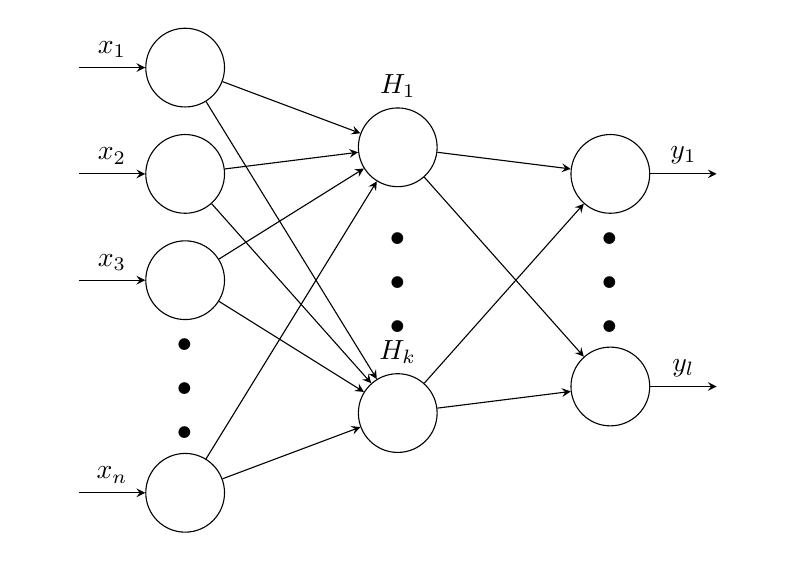
\begin{tikzpicture}[scale=0.9, x=1.5cm, y=1.5cm, >=stealth]

		\foreach \m/\l [count=\y] in {1,2,3,missing,4}
		\node [every neuron/.try, neuron \m/.try] (input-\m) at (0,2.5-\y) {};

		\foreach \m [count=\y] in {1,missing,2}
		\node [every neuron/.try, neuron \m/.try ] (hidden-\m) at (2,2-\y*1.25) {};

		\foreach \m [count=\y] in {1,missing,2}
		\node [every neuron/.try, neuron \m/.try ] (output-\m) at (4,1.5-\y) {};

		\foreach \l [count=\i] in {1,2,3,n}
		\draw [<-] (input-\i) -- ++(-1,0)
		node [above, midway] {$x_\l$};

		\foreach \l [count=\i] in {1,k}
		\node [above] at (hidden-\i.north) {$H_\l$};

		\foreach \l [count=\i] in {1,l}
		\draw [->] (output-\i) -- ++(1,0)
		node [above, midway] {$y_\l$};

		\foreach \i in {1,...,4}
		\foreach \j in {1,...,2}
		\draw [->] (input-\i) -- (hidden-\j);

		\foreach \i in {1,...,2}
		\foreach \j in {1,...,2}
		\draw [->] (hidden-\i) -- (output-\j);
	\end{tikzpicture}
	\begin{equation*}
		f(\mathbf{x};\mathbf{\theta}) = \mathbf{\hat{y}}
	\end{equation*}
\end{frame}

\begin{frame}[c]{Συνελικτικό Δίκτυο}
	\scalebox{0.7}{\begin{tikzpicture}[scale=0.9]
	\draw[dashed] (0.03, 0) -- (1.5, 0);
	\draw[dashed] (1.61, 0) -- (3.01, 0);
	\draw[dashed] (3.2, 0) -- (4.5, 0);
	\draw[dashed] (4.9, 0) -- (6, 0);
	\draw[dashed] (6.8, 0) -- (7.5, 0);
	\networkLayer{4.0}{0.03}{0}{0.0}{color=white}{}
	\networkLayer{3.5}{0.1}{1.5}{0.0}{color=white}{}
	\networkLayer{3.0}{0.2}{3.0}{0.0}{color=white}{}
	\networkLayer{2.5}{0.4}{4.5}{0.0}{color=white}{}
	\networkLayer{2.0}{0.8}{6.0}{0.0}{color=white}{}
	\networkLayer{1.5}{1.6}{7.5}{0.0}{color=white}{}
	\draw[dashed] (10, -1) -- (11.5, 0.5);
	\draw[-] (10.5, -1) -- (12, 0.5);
	\draw[-] (10.5, -0.5) -- (12, 1);
	\draw[-] (10, -0.5) -- (11.5, 1);
	\draw[-] (12, 1) -- (11.5, 1);
	\draw[-] (12, 1) -- (12, 0.5);
	\draw[-] (10, -1) rectangle ++ (0.5,0.5) node{};
	\node[canvas is zy plane at x=0, scale=0.9] at (-0.735, 1.235){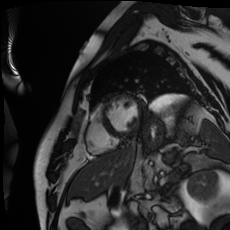
\includegraphics[scale=0.491]{mri_image.png}};
	\node[canvas is zy plane at x=0, scale=0.9] at (0.93, 1.07){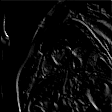
\includegraphics[scale=0.89]{layer_0_feature_map_0.png}};
	\node[canvas is zy plane at x=0, scale=0.9] at (0.83, 1.07){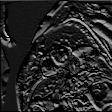
\includegraphics[scale=0.89]{layer_0_feature_map_2.png}};
	\node[canvas is zy plane at x=0, scale=0.9] at (2.63, 0.93){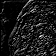
\includegraphics[scale=1.52]{layer_1_feature_map_0.png}};
	\node[canvas is zy plane at x=0, scale=0.9] at (2.42, 0.93){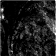
\includegraphics[scale=1.52]{layer_1_feature_map_1.png}};
	\node[canvas is zy plane at x=0, scale=0.9] at (4.42, 0.78){
\includegraphics[scale=2.53]{layer_2_feature_map_0.png}};
	\node[canvas is zy plane at x=0, scale=0.9] at (4.03, 0.78){
\includegraphics[scale=2.53]{layer_2_feature_map_3.png}};
	\node[canvas is zy plane at x=0, scale=0.9] at (6.42, 0.611){
\includegraphics[scale=4.05]{layer_3_feature_map_0.png}};
	\node[canvas is zy plane at x=0, scale=0.9] at (5.6, 0.611){
\includegraphics[scale=4.05]{layer_3_feature_map_2.png}};
	\node[canvas is zy plane at x=0, scale=0.9] at (8.815, 0.472){
\includegraphics[scale=6.05]{layer_4_feature_map_0.png}};
	\node[canvas is zy plane at x=0, scale=0.9] at (7.22, 0.472){
\includegraphics[scale=6.05]{layer_4_feature_map_1.png}};
	\node at (8, 0.472) {$\dots$};
	\node at (6, 0.472) {$\dots$};
	\node[canvas is zy plane at x=0] at (-1, -3){
\includegraphics[scale=10]{layer_4_filter_0.png}};
	\node at (-0.8, -3) {$\dots$};
	\node[canvas is zy plane at x=0] at (-0.6, -3){
\includegraphics[scale=10]{layer_4_filter_1.png}};
	\node[canvas is zy plane at x=0] at (0.8, -3){
\includegraphics[scale=10]{layer_9_filter_0.png}};
	\node at (1, -3) {$\dots$};
	\node[canvas is zy plane at x=0] at (1.3, -3){
\includegraphics[scale=10]{layer_9_filter_1.png}};
	\node[canvas is zy plane at x=0] at (2.5, -3){
\includegraphics[scale=10]{layer_16_filter_0.png}};
	\node at (2.7, -3) {$\dots$};
	\node[canvas is zy plane at x=0] at (2.9, -3){
\includegraphics[scale=10]{layer_16_filter_1.png}};
	\node[canvas is zy plane at x=0] at (4.2, -3){
\includegraphics[scale=10]{layer_23_filter_0.png}};
	\node at (4.4, -3) {$\dots$};
	\node[canvas is zy plane at x=0] at (4.6, -3){
\includegraphics[scale=10]{layer_23_filter_1.png}};
	\node[canvas is zy plane at x=0] at (6.3, -3){
\includegraphics[scale=10]{layer_30_filter_0.png}};
	\node at (6.5, -3) {$\dots$};
	\node[canvas is zy plane at x=0] at (6.7, -3){
\includegraphics[scale=10]{layer_30_filter_1.png}};
	\draw[<-] (-0.3, -3) -- (0.3, -3);
	\draw[<-] (1.6, -3) -- (2.1, -3);
	\draw[<-] (3.2, -3) -- (3.9, -3);
	\draw[<-] (4.8, -3) -- (5.9, -3);
	\draw[<-] (7.1, -3) -- (13.0, -3);
	\draw[dashed] (-1.51, -1.53) -- (0.15, -1.35);
	\draw[dashed] (0.27, -1.35) -- (1.85, -1.16);
	\draw[dashed] (2.05, -1.16) -- (3.55, -0.97);
	\draw[dashed] (3.95, -0.97) -- (5.25, -0.77);
	\draw[dashed] (6.02, -0.78) -- (6.94, -0.57);
	\draw[dashed] (-1.51, 2.45) -- (0.15, 2.15);
	\draw[dashed] (0.27, 2.15) -- (1.85, 1.85);
	\draw[dashed] (2.05, 1.85) -- (3.55, 1.54);
	\draw[dashed] (3.95, 1.54) -- (5.25, 1.23);
	\draw[dashed] (6.02, 1.22) -- (6.94, 0.91);
	\draw[dashed] (0.03, 4) -- (1.5, 3.51);
	\draw[dashed] (1.61, 3.51) -- (3.01, 3.01);
	\draw[dashed] (3.2, 3) -- (4.5, 2.5);
	\draw[dashed] (4.9, 2.51) -- (6, 2);
	\draw[dashed] (6.8, 2) -- (7.5, 1.5);
	\draw[dotted] (9.1, 1.5) --(11.5, 1);
	\draw[dotted] (9.1, 0) -- (11.5, 0.5);
	\draw[dotted] (8.5, 0.92) -- (10, -0.5);
	\draw[dotted] (8.5, -0.58) --  (10, -1);
	\draw[dashdotted] (10.5, -0.5) -- (13, -0.25);
	\draw[dashdotted] (10.5, -1) -- (13, -0.25);
	\draw[dashdotted] (12, 1) -- (13, -0.25);
	\draw[dashdotted] (12, 0.5) -- (13, -0.25);
	\node[align=left] at (13.3,-0.2) {$\hat{y}$};
	\draw[->] (13.3, -0.6) -- (13.3, -2.7) node [pos=1.1] {$J$};
	\draw[<-] (13.5, -3) -- (14, -3) node [pos=1.6] {$y$};
	\node[align=left] at (10.0, -2.4) {αντίστροφη διάδοση σφάλματος};
	\node[align=left] at (10.8, 2.5) {προς-τα-εμπρός διάδοση};
\end{tikzpicture}
}
\end{frame}

\section{Επίπεδα \textlatin{Signal2Image}}
\begin{frame}[c]{Αρχιτεκτονική \textlatin{Signal2Image}}
	\scalebox{1.2}{
		\begin{tikzpicture}[]
			\node[] at (-4.5, 0){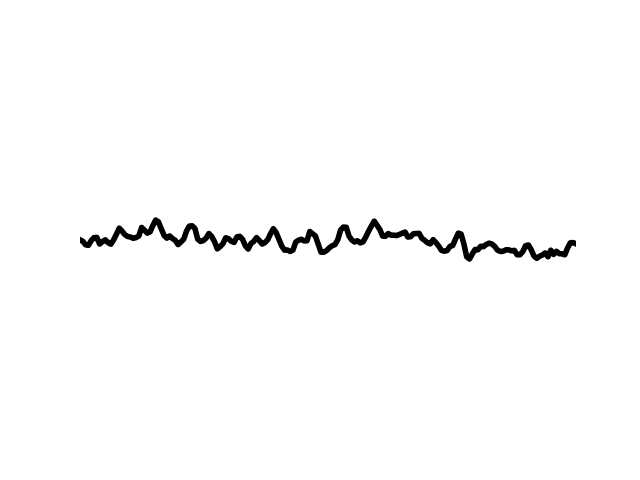
\includegraphics[scale=0.2,angle=90]{signal_epilepsy.png}};
			\node[align=left] at (-4.2, 0) {$x_i$};
			\draw[dashed,->] (-4, 0) -- (-3.8, 0);
			\node[draw, minimum height=2.55cm] at (-3.5, 0) {$m$};
			\draw[dashed,->] (-3.2, 0) -- (-3, 0);
			\node[] at (-1.7, 0){
\includegraphics[scale=0.41,angle=90]{cnn_epilepsy.png}};
			\draw[dashed,->] (-0.4, 0) -- (-0.2, 0);
			\node[draw, minimum height=2.55cm] at (0.1, 0) {$b_{d}$};
			\draw[dashed,->] (0.4, 0) -- (0.6, 0);
			\node[align=left] at (0.8, 0) {$\hat{y_i}$};
			\node[minimum width=0.5cm, minimum height=0.5cm] at (2, 1.1) {\footnotesize \textlatin{Open} 0.1\%};
			\node[minimum width=0.5cm, minimum height=0.5cm] at (2, 0.55) {\footnotesize \textlatin{Closed} 0.2\%};
			\node[minimum width=0.5cm, minimum height=0.5cm] at (2, 0) {\footnotesize \textlatin{Healthy} 0.9\%};
			\node[minimum width=0.5cm, minimum height=0.5cm] at (2, -0.55) {\footnotesize \textlatin{Tumor} 34.7\%};
			\node[minimum width=0.5cm, minimum height=0.5cm] at (2, -1.1) {\footnotesize \textlatin{Epilepsy} 64.1\%};
		\end{tikzpicture}
		}
\end{frame}

\begin{frame}[c]{Ενδιάμεσες Αναπαραστάσεις}
	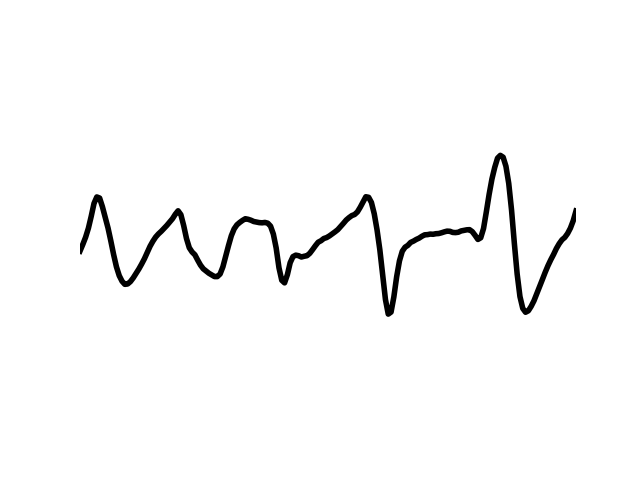
\includegraphics[scale=0.1]{signal_eyes_open.png}
	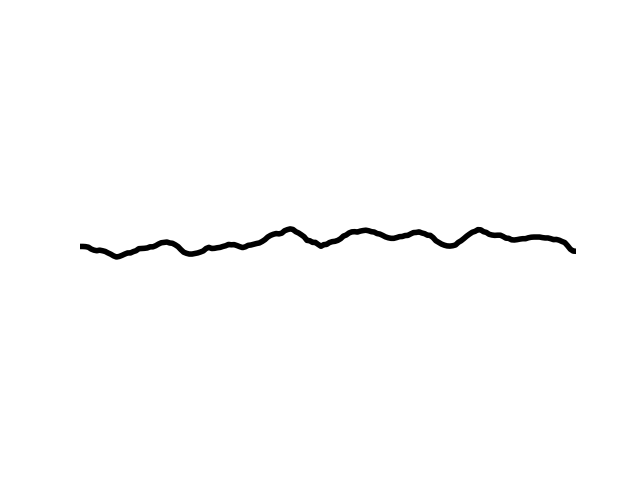
\includegraphics[scale=0.1]{signal_eyes_closed.png}
	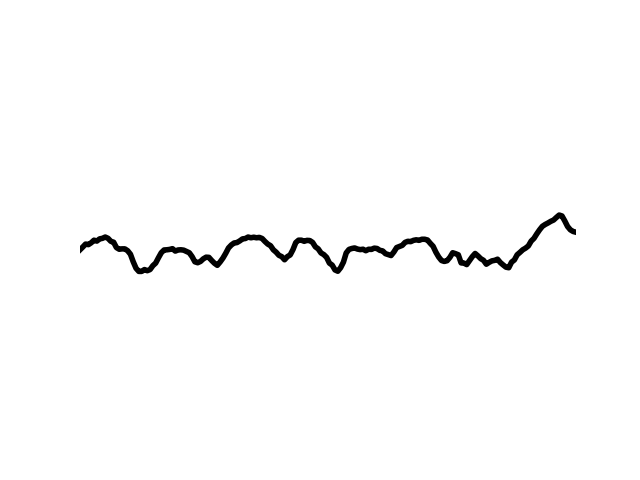
\includegraphics[scale=0.1]{signal_healthy_area.png}
	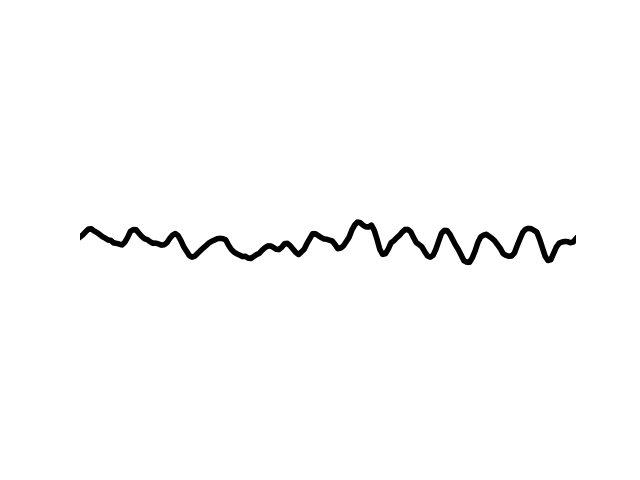
\includegraphics[scale=0.1]{signal_tumor_area.png}
	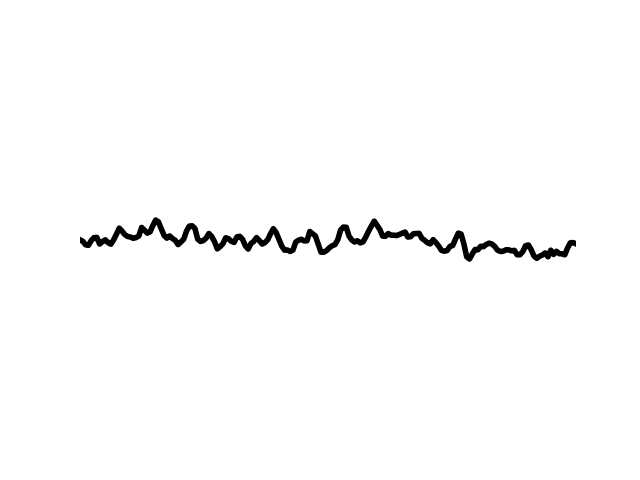
\includegraphics[scale=0.1]{signal_epilepsy.png}
	\\
	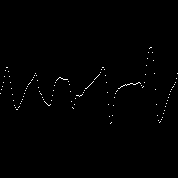
\includegraphics[scale=0.26]{signal_as_image_eyes_open.png}
	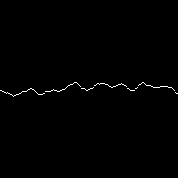
\includegraphics[scale=0.26]{signal_as_image_eyes_closed.png}
	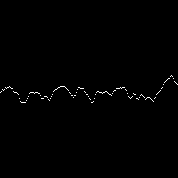
\includegraphics[scale=0.26]{signal_as_image_healthy_area.png}
	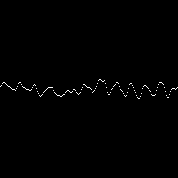
\includegraphics[scale=0.26]{signal_as_image_tumor_area.png}
	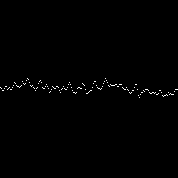
\includegraphics[scale=0.26]{signal_as_image_epilepsy.png}
	\\
	
\includegraphics[scale=0.26]{spectrogram_eyes_open.png}
	
\includegraphics[scale=0.26]{spectrogram_eyes_closed.png}
	
\includegraphics[scale=0.26]{spectrogram_healthy_area.png}
	
\includegraphics[scale=0.26]{spectrogram_tumor_area.png}
	
\includegraphics[scale=0.26]{spectrogram_epilepsy.png}
	\\
	
\includegraphics[scale=0.26]{cnn_eyes_open.png}
	
\includegraphics[scale=0.26]{cnn_eyes_closed.png}
	
\includegraphics[scale=0.26]{cnn_healthy_area.png}
	
\includegraphics[scale=0.26]{cnn_tumor_area.png}
	
\includegraphics[scale=0.26]{cnn_epilepsy.png}
\end{frame}

\begin{frame}[c]{Αποτελέσματα}
	\begin{table}
		\scalebox{0.46}{
			\textlatin{
				\begin{tabular}{l | c | c | c c c c | c c c c c | c c c c }
	\toprule
	\multirow{2}{*}{\diagbox{Dim, S2I}{Model}} & LeNet         & AlexNet       & \multicolumn{4}{c|}{VGGnet} & \multicolumn{5}{c|}{ResNet} & \multicolumn{4}{c}{DenseNet}                                                                                                                                                                 \\
	& 2             & 5             & 11                          & 13                          & 16                           & 19            & 18            & 34            & 50            & 101           & 152           & 121           & 161           & 169           & 201           \\
	\midrule
	1D, none                                   & 72.6          & 78.8          & 76.9                        & \textbf{79.0}               & 79.5                         & \textbf{79.3} & 81.5          & 82.5          & 81.4          & 78.8          & 81.4          & 81.8          & \textbf{83.3} & 82.1          & 82.0          \\
	\midrule
	2D, signal as image                        & 67.9          & 68.3          & 74.1                        & 74.7                        & 72.7                         & 72.5          & 73.3          & 71.7          & 74.1          & 72.3          & 74.1          & 74.7          & 72.5          & 75.2          & 75.0          \\
	\midrule
	2D, spectrogram                            & 73.2          & 74.0          & 77.9                        & 76.3                        & 77.5                         & 76.0          & 76.2          & 79.0          & 77.2          & 74.6          & 75.3          & 74.1          & 75.2          & 77.0          & 75.4          \\
	\midrule
	2D, one layer CNN                          & \textbf{75.8} & \textbf{82.0} & \textbf{84.0}               & 77.9                        & 80.7                         & 78.4          & \textbf{85.1} & \textbf{84.6} & \textbf{83.0} & \textbf{85.0} & \textbf{83.3} & \textbf{84.3} & 80.7          & \textbf{85.0} & \textbf{85.3} \\
	\midrule
	2D, two layer CNN                          & 75.0          & 77.9          & 80.7                        & 78.8                        & \textbf{81.1}                & 74.9          & 78.3          & 80.0          & 78.3          & 77.1          & 80.9          & 83.2          & 82.3          & 79.0          & 79.1          \\
	\bottomrule
\end{tabular}

				}
				}
	\end{table}
\end{frame}

\section{Μέτρο $\varphi$}
\begin{frame}[c]{$\varphi$}
	\begin{columns}
		\begin{column}{0.5\textwidth}
			\begin{equation*}
				W = \sum\limits_{i=1}^q m^{(i)}
			\end{equation*}
			\begin{equation*}
				A_{\bm{x}} = \sum\limits_{i=1}^q \left\Vert\bm{\alpha}^{(i)}\right\Vert_0
			\end{equation*}
			\begin{equation*}
				CR = \frac{n}{W + (\dim(\bm{x}) + 1)A_{\bm{x}}}
			\end{equation*}
		\end{column}
		\begin{column}{0.5\textwidth}
			\begin{equation*}
				\tilde{\mathcal{L}}(\hat{\bm{x}},\bm{x}) = \frac{\mathcal{L}(\hat{\bm{x}},\bm{x})}{\mathcal{L}(0,\bm{x})}
			\end{equation*}
			\begin{equation*}
				\varphi = \lVert\left(CR^{-1}, \tilde{\mathcal{L}}(\hat{\bm{x}},\bm{x})\right)\rVert_2
			\end{equation*}
			\begin{equation*}
				\bar\varphi = \frac{1}{l}\sum\limits_{j=1}^l \varphi^{(j)}
			\end{equation*}
		\end{column}
	\end{columns}
\end{frame}

\section{Συναρτήσεις Αραιής Ενεργοποίησης}
\begin{frame}[c]{Συναρτήσεις Αραιής Ενεργοποίησης}
	\begin{columns}
		\begin{column}{0.5\textwidth}
			\begin{algorithm}[H]
				\floatname{algorithm}{Αλγόριθμος}
				\caption{Ταυτότητα}
				\textlatin{
					\begin{algorithmic}[1]
						\renewcommand{\algorithmicrequire}{\textbf{Input:}}
						\renewcommand{\algorithmicensure}{\textbf{Output:}}
						\REQUIRE $s$
						\RETURN $s$
					\end{algorithmic}
					}
			\end{algorithm}
		\end{column}
		\begin{column}{0.5\textwidth}
			\begin{figure}
				\includegraphics[width=0.6\textwidth]{"images_1d/UCI-epilepsy_identity_1d_2_activations_0"}
				\\
				\includegraphics[width=0.6\textwidth]{"images_2d/MNIST_identity_2d_2_activations_1"}
			\end{figure}
		\end{column}
	\end{columns}
\end{frame}

\begin{frame}[c]{Συναρτήσεις Αραιής Ενεργοποίησης}
	\begin{columns}
		\begin{column}{0.5\textwidth}
			\begin{algorithm}[H]
				\floatname{algorithm}{Αλγόριθμος}
				\caption{\textlatin{ReLU}}
				\textlatin{
					\begin{algorithmic}[1]
						\renewcommand{\algorithmicrequire}{\textbf{Input:}}
						\renewcommand{\algorithmicensure}{\textbf{Output:}}
						\REQUIRE $s$
						\ENSURE $u$
						\FOR {$i$ = 0 to $|s|$}
						\IF {$s_i > 0$}
						\STATE $u_i = s_i$
						\ELSE
						\STATE $u_i = 0$
						\ENDIF
						\ENDFOR
						\RETURN $u$
					\end{algorithmic}
					}
			\end{algorithm}
		\end{column}
		\begin{column}{0.5\textwidth}
			\begin{figure}
				\includegraphics[width=0.6\textwidth]{"images_1d/UCI-epilepsy_relu_1d_2_activations_0"}
				\\
				\includegraphics[width=0.6\textwidth]{"images_2d/MNIST_relu_2d_2_activations_0"}
			\end{figure}
		\end{column}
	\end{columns}
\end{frame}

\begin{frame}[c]{Συναρτήσεις Αραιής Ενεργοποίησης}
	\begin{columns}
		\begin{column}{0.5\textwidth}
			\begin{algorithm}[H]
				\floatname{algorithm}{Αλγόριθμος}
				\caption{κ-μέγιστα απολύτων}
				\textlatin{
					\begin{algorithmic}[1]
	\renewcommand{\algorithmicrequire}{\textbf{Input:}}
	\renewcommand{\algorithmicensure}{\textbf{Output:}}
	\REQUIRE $s$, $k$
	\ENSURE $\alpha$
	\STATE $\alpha_i \leftarrow 0, i=1\ldots card(s)$
	\STATE $p \leftarrow topk(\lvert s\rvert, k)$
	\FOR {$i$ = 0 to $card(s)$}
	\STATE $\alpha_i(p_i) = s_i(p_i)$
	\ENDFOR
	\RETURN $\alpha$
\end{algorithmic}

					}
			\end{algorithm}
		\end{column}
		\begin{column}{0.5\textwidth}
			\begin{figure}
				\includegraphics[width=0.6\textwidth]{"images_1d/UCI-epilepsy_topk_absolutes_1d_2_activations_0"}
				\\
				\includegraphics[width=0.6\textwidth]{"images_2d/MNIST_topk_absolutes_2d_2_activations_0"}
			\end{figure}
		\end{column}
	\end{columns}
\end{frame}

\begin{frame}[c]{Συναρτήσεις Αραιής Ενεργοποίησης}
	\begin{columns}
		\begin{column}{0.5\textwidth}
			\begin{algorithm}[H]
				\floatname{algorithm}{Αλγόριθμος}
				\caption{Δείκτες Συγκέντρωσης Ακρότατων}
				\textlatin{
					\begin{algorithmic}[1]
	\renewcommand{\algorithmicrequire}{\textbf{Input:}}
	\renewcommand{\algorithmicensure}{\textbf{Output:}}
	\REQUIRE $s$, $m$
	\ENSURE $\alpha$
	\STATE $p \leftarrow maxpool(\lvert s\rvert, m)$
	\STATE $\alpha \leftarrow maxunpool(s(p), p, m)$
	\RETURN $\alpha$
\end{algorithmic}

					}
			\end{algorithm}
		\end{column}
		\begin{column}{0.5\textwidth}
			\begin{figure}
				\includegraphics[width=0.6\textwidth]{"images_1d/UCI-epilepsy_extrema_pool_indices_1d_2_activations_0"}
				\\
				\includegraphics[width=0.6\textwidth]{"images_2d/MNIST_extrema_pool_indices_2d_2_activations_0"}
			\end{figure}
		\end{column}
	\end{columns}
\end{frame}

\begin{frame}[c]{Συναρτήσεις Αραιής Ενεργοποίησης}
	\begin{columns}
		\begin{column}{0.6\textwidth}
			\scalebox{0.6}{
				\begin{minipage}{\linewidth}
					\begin{algorithm}[H]
						\floatname{algorithm}{Αλγόριθμος}
						\caption{Ακρότατα}
						\textlatin{
							\begin{algorithmic}[1]
	\renewcommand{\algorithmicrequire}{\textbf{Input:}}
	\renewcommand{\algorithmicensure}{\textbf{Output:}}
	\REQUIRE $s$, $med$
	\ENSURE $\alpha$
	\STATE $peaks \leftarrow \left(\frac{d s}{d t}^+ \geq 0\right) \land \left(\frac{d s}{d t}^- < 0\right)$
	\STATE $valleys \leftarrow \left(\frac{d s}{d t}^+ < 0\right) \land \left(\frac{d s}{d t}^- \geq 0\right)$ \\
	\textit{\scriptsize \# + and - denote one sample padding to the right and left respectively}
	\STATE $z = peaks \lor valleys$
	\STATE $p_i \leftarrow z > 0$
	\STATE $p_{i_i} \leftarrow sort(z)$
	\STATE $p_{i_{sorted}} \leftarrow p_i(p_{i_i})$
	\STATE $q_i \leftarrow 0, i=1\ldots card(s)$
	\FOR {$i$ = 0 to $card(s)$}
	\IF {$\lnot q_i$}
	\STATE $p_{i_r} \leftarrow p_i \geq p_{i_i} - med$
	\STATE $p_{i_l} \leftarrow p_i \leq p_{i_i} + med$
	\STATE $p_{i_m} \leftarrow p_{i_r} \land p_{i_l}$
	\STATE $q \leftarrow q \lor p_{i_m}$
	\STATE $q_i \leftarrow 0$
	\ENDIF
	\ENDFOR
	\STATE $\alpha_{ind} \leftarrow p_{i_{sorted}}(\lnot q)$
	\STATE $\alpha_i \leftarrow 0, i=1\ldots card(s)$
	\STATE $\alpha(\alpha_i) \leftarrow s(\alpha_{ind})$
	\RETURN $\alpha$
\end{algorithmic}

							}
					\end{algorithm}
				\end{minipage}
				}
		\end{column}
		\begin{column}{0.4\textwidth}
			\begin{minipage}{\linewidth}
				\includegraphics[width=0.8\textwidth]{"images_1d/UCI-epilepsy_extrema_1d_2_activations_0"}
				\\
				\includegraphics[width=0.8\textwidth]{"images_2d/MNIST_extrema_2d_2_activations_0"}
			\end{minipage}
		\end{column}
	\end{columns}
\end{frame}

\section{Δίκτυα Αραιής Ενεργοποίησης}
\begin{frame}[c]{Δίκτυα Αραιής Ενεργοποίησης}
	\framesubtitle{Αρχιτεκτονική}
	\begin{figure}
		\begin{tikzpicture}[scale=0.6]
			\begin{scope}[tdplot_main_coords, canvas is yz plane at x=-0.5,xscale=-1, transform shape]
	\node[opacity=0] at (0, 0)(input){\includegraphics[scale=\figscale]{"images_1d/UCI-epilepsy_extrema_1d_2_signal"}};
	\node[opacity=0, draw, right=0.5cm of input, circle] (loss){$\mathcal{L}$};
	\node[opacity=0, right=0.5cm of loss] (reconstructed){\includegraphics[scale=\figscale]{"images_1d/UCI-epilepsy_extrema_1d_2_reconstructed"}};
	\node[opacity=0, draw, below=0.5cm of reconstructed, circle] (plus){$+$};
	\node[opacity=0.8, below=0.5cm of plus] (reconstruction){\includegraphics[scale=\figscale]{"images_1d/UCI-epilepsy_extrema_1d_2_reconstruction_0"}};
	\node[opacity=0, draw, below=0.5cm of reconstruction, circle] (conv2){$\ast$};
	\node[] at (4.8, -3.4){$\bm{r}^{(0)}$};
	\node[opacity=0.8, below=0.5cm of conv2] (extrema){\includegraphics[scale=\figscale]{"images_1d/UCI-epilepsy_extrema_1d_2_activations_0"}};
	\node[opacity=0, draw, left=0.55cm of extrema, circle] (phi){$\phi$};
	\node[] at (4.8, -7.4){$\bm{\alpha}^{(0)}$};
	\node[opacity=0.8, left=0.55cm of phi] (similarity){\includegraphics[scale=\figscale]{"images_1d/UCI-epilepsy_extrema_1d_2_similarity_0"}};
	\node[] at (0.1, -7.4){$\bm{s}^{(0)}$};
	\node[left=1.5cm of conv2] (kernel){\includegraphics[scale=0.1]{"images_1d/UCI-epilepsy_extrema_1d_2_kernel_0"}};
	\node[] at (2.6, -5.6){\tiny $\bm{w}^{(0)}$};
	\node[opacity=0, draw, above=0.5cm of similarity, circle] (conv1){$\ast$};
\end{scope}
\begin{scope}[tdplot_main_coords, canvas is yz plane at x=0,xscale=-1, transform shape]
	\node[] at (0, 0)(input){\includegraphics[scale=\figscale]{"images_1d/UCI-epilepsy_extrema_1d_2_signal"}};
	\node[] at (0.1, 0.7){$\bm{x}$};
	\node[draw, right=0.5cm of input, circle] (loss){$\mathcal{L}$};
	\node[right=0.5cm of loss] (reconstructed){\includegraphics[scale=\figscale]{"images_1d/UCI-epilepsy_extrema_1d_2_reconstructed"}};
	\node[] at (4.8, 0.7){$\hat{\bm{x}}$};
	\node[draw, below=0.5cm of reconstructed, circle] (plus){$+$};
	\node[opacity=0, below=0.5cm of plus] (reconstruction){\includegraphics[scale=\figscale]{"images_1d/UCI-epilepsy_extrema_1d_2_reconstruction_0"}};
	\node[draw, below=0.5cm of reconstruction, circle] (conv2){$\ast$};
	\node[opacity=0, below=0.5cm of conv2] (extrema){\includegraphics[scale=\figscale]{"images_1d/UCI-epilepsy_extrema_1d_2_activations_0"}};
	\node[draw, left=0.55cm of extrema, circle, inner sep=2pt] (phi){$\phi$};
	\node[opacity=0, left=0.55cm of phi] (similarity){\includegraphics[scale=\figscale]{"images_1d/UCI-epilepsy_extrema_1d_2_similarity_0"}};
	\node[opacity=0, left=1.5cm of conv2] (kernel){\includegraphics[scale=0.1]{"images_1d/UCI-epilepsy_extrema_1d_2_kernel_0"}};
	\node[draw, above=0.5cm of similarity, circle] (conv1){$\ast$};
	\draw[->](input) -- node{} (conv1);
	\draw[->](conv1) -- node{} (similarity);
	\draw[->](similarity) -- node{} (phi);
	\draw[->](phi) -- node{} (extrema);
	\draw[->](extrema) -- node{} (conv2);
	\draw[->](conv2) -- node{} (reconstruction);
	\draw[->](reconstruction) -- node{} (plus);
	\draw[->](plus) -- node{} (reconstructed);
	\draw[->](kernel) -- node{} (conv1);
	\draw[->](kernel) -- node{} (conv2);
	\draw[->](input) -- node{} (loss);
	\draw[->](reconstructed) -- node{} (loss);
\end{scope}
\begin{scope}[tdplot_main_coords, canvas is yz plane at x=0.5,xscale=-1, transform shape]
	\node[opacity=0] at (0, 0)(input){\includegraphics[scale=\figscale]{"images_1d/UCI-epilepsy_extrema_1d_2_signal"}};
	\node[opacity=0, draw, right=0.5cm of input, circle] (loss){$\mathcal{L}$};
	\node[opacity=0, right=0.5cm of loss] (reconstructed){\includegraphics[scale=\figscale]{"images_1d/UCI-epilepsy_extrema_1d_2_reconstructed"}};
	\node[opacity=0, draw, below=0.5cm of reconstructed, circle] (plus){$+$};
	\node[opacity=0.8, below=0.5cm of plus] (reconstruction){\includegraphics[scale=\figscale]{"images_1d/UCI-epilepsy_extrema_1d_2_reconstruction_1"}};
	\node[] at (4.8, -3.4){$\bm{r}^{(1)}$};
	\node[opacity=0, draw, below=0.5cm of reconstruction, circle] (conv2){$\ast$};
	\node[opacity=0.8, below=0.5cm of conv2] (extrema){\includegraphics[scale=\figscale]{"images_1d/UCI-epilepsy_extrema_1d_2_activations_1"}};
	\node[] at (4.8, -7.4){$\bm{\alpha}^{(1)}$};
	\node[opacity=0, draw, left=0.55cm of extrema, circle] (phi){$\phi$};
	\node[opacity=0.8, left=0.55cm of phi] (similarity){\includegraphics[scale=\figscale]{"images_1d/UCI-epilepsy_extrema_1d_2_similarity_1"}};
	\node[] at (0.1, -7.4){$\bm{s}^{(1)}$};
	\node[left=1.5cm of conv2] (kernel){\includegraphics[scale=0.1]{"images_1d/UCI-epilepsy_extrema_1d_2_kernel_1"}};
	\node[] at (2.6, -5.6){\tiny $\bm{w}^{(1)}$};
	\node[opacity=0, draw, above=0.5cm of similarity, circle] (conv1){$\ast$};
\end{scope}

		\end{tikzpicture}
		\qquad
		\begin{tikzpicture}[scale=0.6]
			\begin{scope}[tdplot_main_coords, canvas is yz plane at x=-0.5,xscale=-1, transform shape]
	\node[opacity=0] at (0, 0)(input){\includegraphics[scale=\figscale]{"images_2d/MNIST_extrema_2d_2_signal"}};
	\node[opacity=0, draw, right=0.5cm of input, circle] (loss){$\mathcal{L}$};
	\node[opacity=0, right=0.5cm of loss] (reconstructed){\includegraphics[scale=\figscale]{"images_2d/MNIST_extrema_2d_2_reconstructed"}};
	\node[opacity=0, draw, below=0.5cm of reconstructed, circle] (plus){$+$};
	\node[opacity=0.8, below=0.5cm of plus] (reconstruction){\includegraphics[scale=\figscale]{"images_2d/MNIST_extrema_2d_2_reconstruction_0"}};
	\node[opacity=0, draw, below=0.5cm of reconstruction, circle] (conv2){$\ast$};
	\node[opacity=0.8, below=0.5cm of conv2] (extrema){\includegraphics[scale=\figscale]{"images_2d/MNIST_extrema_2d_2_activations_0"}};
	\node[opacity=0, draw, left=0.55cm of extrema, circle] (phi){$\phi$};
	\node[opacity=0.8, left=0.55cm of phi] (similarity){\includegraphics[scale=\figscale]{"images_2d/MNIST_extrema_2d_2_similarity_0"}};
	\node[opacity=0.8, left=1.2cm of conv2] (kernel){\includegraphics[scale=0.1]{"images_2d/MNIST_extrema_2d_2_kernel_0"}};
	\node[opacity=0, draw, above=0.5cm of similarity, circle] (conv1){$\ast$};
\end{scope}
\begin{scope}[tdplot_main_coords, canvas is yz plane at x=0,xscale=-1, transform shape]
	\node[] at (0, 0)(input){\includegraphics[scale=\figscale]{"images_2d/MNIST_extrema_2d_2_signal"}};
	\node[draw, right=0.5cm of input, circle] (loss){$\mathcal{L}$};
	\node[right=0.5cm of loss] (reconstructed){\includegraphics[scale=\figscale]{"images_2d/MNIST_extrema_2d_2_reconstructed"}};
	\node[draw, below=0.5cm of reconstructed, circle] (plus){$+$};
	\node[opacity=0, below=0.5cm of plus] (reconstruction){\includegraphics[scale=\figscale]{"images_2d/MNIST_extrema_2d_2_reconstruction_0"}};
	\node[draw, below=0.5cm of reconstruction, circle] (conv2){$\ast$};
	\node[opacity=0, below=0.5cm of conv2] (extrema){\includegraphics[scale=\figscale]{"images_2d/MNIST_extrema_2d_2_activations_0"}};
	\node[draw, left=0.55cm of extrema, circle, inner sep=2pt] (phi){$\phi$};
	\node[opacity=0, left=0.55cm of phi] (similarity){\includegraphics[scale=\figscale]{"images_2d/MNIST_extrema_2d_2_similarity_0"}};
	\node[opacity=0, left=1.2cm of conv2] (kernel){\includegraphics[scale=0.1]{"images_2d/MNIST_extrema_2d_2_kernel_0"}};
	\node[draw, above=0.5cm of similarity, circle] (conv1){$\ast$};
	\draw[->](input) -- node{} (conv1);
	\draw[->](conv1) -- node{} (similarity);
	\draw[->](similarity) -- node{} (phi);
	\draw[->](phi) -- node{} (extrema);
	\draw[->](extrema) -- node{} (conv2);
	\draw[->](conv2) -- node{} (reconstruction);
	\draw[->](reconstruction) -- node{} (plus);
	\draw[->](plus) -- node{} (reconstructed);
	\draw[->](kernel) -- node{} (conv1);
	\draw[->](kernel) -- node{} (conv2);
	\draw[->](input) -- node{} (loss);
	\draw[->](reconstructed) -- node{} (loss);
\end{scope}
\begin{scope}[tdplot_main_coords, canvas is yz plane at x=0.5,xscale=-1, transform shape]
	\node[opacity=0] at (0, 0)(input){\includegraphics[scale=\figscale]{"images_2d/MNIST_extrema_2d_2_signal"}};
	\node[opacity=0, draw, right=0.5cm of input, circle] (loss){$\mathcal{L}$};
	\node[opacity=0, right=0.5cm of loss] (reconstructed){\includegraphics[scale=\figscale]{"images_2d/MNIST_extrema_2d_2_reconstructed"}};
	\node[opacity=0, draw, below=0.5cm of reconstructed, circle] (plus){$+$};
	\node[opacity=0.8, below=0.5cm of plus] (reconstruction){\includegraphics[scale=\figscale]{"images_2d/MNIST_extrema_2d_2_reconstruction_1"}};
	\node[opacity=0, draw, below=0.5cm of reconstruction, circle] (conv2){$\ast$};
	\node[opacity=0.8, below=0.5cm of conv2] (extrema){\includegraphics[scale=\figscale]{"images_2d/MNIST_extrema_2d_2_activations_1"}};
	\node[opacity=0, draw, left=0.55cm of extrema, circle] (phi){$\phi$};
	\node[opacity=0.8, left=0.55cm of phi] (similarity){\includegraphics[scale=\figscale]{"images_2d/MNIST_extrema_2d_2_similarity_1"}};
	\node[opacity=0.8, left=1.2cm of conv2] (kernel){\includegraphics[scale=0.1]{"images_2d/MNIST_extrema_2d_2_kernel_1"}};
	\node[opacity=0, draw, above=0.5cm of similarity, circle] (conv1){$\ast$};
\end{scope}

		\end{tikzpicture}
	\end{figure}
\end{frame}

\begin{frame}[c]{Αλγόριθμος Εκπαίδευσης \textlatin{SANs}}
	\begin{center}
		\scalebox{0.6}{
			\begin{minipage}{\linewidth}
				\begin{algorithm}[H]
					\floatname{algorithm}{Αλγόριθμος}
					\caption{Εκπαίδευση δικτύων αραιής ενεργοποίησης}
					\textlatin{
						\begin{algorithmic}[1]
	\renewcommand{\algorithmicrequire}{\textbf{Input:}}
	\renewcommand{\algorithmicensure}{\textbf{Output:}}
	\REQUIRE $\bm{x}$
	\ENSURE $\bm{\alpha}$, $\bm{w}$
	\\ \textit{Hyperparameters:  $m$, $\mu$, $\sigma$, $q$, $\phi$, $d$, $\lambda$, $epochs$, $batches$}
	\FOR {$i$ = 1 to $q$}
	\STATE $\bm{w}^{(i)} \sim \mathcal{N}(\mu, \sigma)$
	\ENDFOR
	\FOR {$e$ = 1 to $epochs$}
	\FOR {$b$ = 1 to $batches$}
	\STATE $\bm{x}^{(b)} \sim \bm{x}$
	\FOR {$i$ = 1 to $q$}
	\STATE $\bm{s}^{(i)} \leftarrow \bm{x}^{(b)} * \bm{w}^{(i)}$
	\STATE $\bm{\alpha}^{(i)} \leftarrow \phi(\bm{s}^{(i)}, d^{(i)})$
	\STATE $r^{(i)} \leftarrow \bm{\alpha}^{(i)} * \bm{w}^{(i)}$
	\ENDFOR
	\STATE $\hat{\bm{x}}^{(b)} \leftarrow \sum\limits_{i=1}^q r^{(i)}$
	\STATE $\mathcal{L} \leftarrow \frac{1}{n}\sum\limits_{t=1}^n \lvert\hat{\bm{x}}^{(b)}_t - \bm{x}^{(b)}_t \rvert$
	\STATE $\nabla\mathcal{L} = \left( \frac{\partial\mathcal{L}}{\partial\bm{w}^{(1)}},\ldots\frac{\partial\mathcal{L}}{\partial\bm{w}^{(q)}}\right)$
	\STATE $\Delta\bm{w}^{(i)} = -\lambda\frac{\partial\mathcal{L}}{\partial\bm{w}^{(i)}}$
	\ENDFOR
	\ENDFOR
	\RETURN $\bm{\alpha}$, $\bm{w}$
\end{algorithmic}

						}
				\end{algorithm}


			\end{minipage}
			}
	\end{center}
\end{frame}

\begin{frame}[c]{$CR^{-1}$ \textlatin{vs}. $\tilde{\mathcal{L}}$}
	\includegraphics[width=0.49\textwidth]{"images_mean_inverse_compression_ratio_vs_mean_reconstruction_loss_variable_kernel_size_list/apnea-ecg"}
	\includegraphics[width=0.49\textwidth]{"images_mean_inverse_compression_ratio_vs_mean_reconstruction_loss_variable_kernel_size_list/legend"}
\end{frame}

\begin{frame}[c]{$CR^{-1}$ \textlatin{vs}. $\tilde{\mathcal{L}}$}
	\includegraphics[width=0.19\textwidth]{"images_mean_inverse_compression_ratio_vs_mean_reconstruction_loss_variable_kernel_size_list/apnea-ecg"}
	\includegraphics[width=0.19\textwidth]{"images_mean_inverse_compression_ratio_vs_mean_reconstruction_loss_variable_kernel_size_list/bidmc"}
	\includegraphics[width=0.19\textwidth]{"images_mean_inverse_compression_ratio_vs_mean_reconstruction_loss_variable_kernel_size_list/bpssrat"}
	\includegraphics[width=0.19\textwidth]{"images_mean_inverse_compression_ratio_vs_mean_reconstruction_loss_variable_kernel_size_list/cebsdb"}
	\includegraphics[width=0.19\textwidth]{"images_mean_inverse_compression_ratio_vs_mean_reconstruction_loss_variable_kernel_size_list/ctu-uhb-ctgdb"}
	\\
	\includegraphics[width=0.19\textwidth]{"images_mean_inverse_compression_ratio_vs_mean_reconstruction_loss_variable_kernel_size_list/drivedb"}
	\includegraphics[width=0.19\textwidth]{"images_mean_inverse_compression_ratio_vs_mean_reconstruction_loss_variable_kernel_size_list/emgdb"}
	\includegraphics[width=0.19\textwidth]{"images_mean_inverse_compression_ratio_vs_mean_reconstruction_loss_variable_kernel_size_list/mitdb"}
	\includegraphics[width=0.19\textwidth]{"images_mean_inverse_compression_ratio_vs_mean_reconstruction_loss_variable_kernel_size_list/noneeg"}
	\includegraphics[width=0.19\textwidth]{"images_mean_inverse_compression_ratio_vs_mean_reconstruction_loss_variable_kernel_size_list/prcp"}
	\\
	\includegraphics[width=0.19\textwidth]{"images_mean_inverse_compression_ratio_vs_mean_reconstruction_loss_variable_kernel_size_list/shhpsgdb"}
	\includegraphics[width=0.19\textwidth]{"images_mean_inverse_compression_ratio_vs_mean_reconstruction_loss_variable_kernel_size_list/slpdb"}
	\includegraphics[width=0.19\textwidth]{"images_mean_inverse_compression_ratio_vs_mean_reconstruction_loss_variable_kernel_size_list/sufhsdb"}
	\includegraphics[width=0.19\textwidth]{"images_mean_inverse_compression_ratio_vs_mean_reconstruction_loss_variable_kernel_size_list/voiced"}
	\includegraphics[width=0.19\textwidth]{"images_mean_inverse_compression_ratio_vs_mean_reconstruction_loss_variable_kernel_size_list/wrist"}
\end{frame}

\begin{frame}[c]{$CR^{-1}$ \textlatin{vs}. $\tilde{\mathcal{L}}$}
	\framesubtitle{διάγραμμα πυκνότητας}
	\includegraphics[width=0.5\textwidth]{"images_1d/crrl_density_plot"}
\end{frame}

\begin{frame}[c]{$\bar\varphi$ \textlatin{vs}. $epochs$, $m$}
	\framesubtitle{διαστήματα εμπιστοσύνης}
	\includegraphics[width=0.49\textwidth]{"images_1d/mean_flethos_validation_epochs"}
	\includegraphics[width=0.49\textwidth]{"images_1d/mean_flethos_variable_kernel_size_list"}
\end{frame}

\begin{frame}[c]{Οπτικοποίηση πυρήνων}
	\includegraphics[width=0.056\textwidth]{"images_1d/apnea-ecg_relu_1d_1_kernel_0"}
\includegraphics[width=0.056\textwidth]{"images_1d/bidmc_relu_1d_1_kernel_0"}
\includegraphics[width=0.056\textwidth]{"images_1d/bpssrat_relu_1d_1_kernel_0"}
\includegraphics[width=0.056\textwidth]{"images_1d/cebsdb_relu_1d_1_kernel_0"}
\includegraphics[width=0.056\textwidth]{"images_1d/ctu-uhb-ctgdb_relu_1d_1_kernel_0"}
\includegraphics[width=0.056\textwidth]{"images_1d/drivedb_relu_1d_1_kernel_0"}
\includegraphics[width=0.056\textwidth]{"images_1d/emgdb_relu_1d_1_kernel_0"}
\includegraphics[width=0.056\textwidth]{"images_1d/mitdb_relu_1d_1_kernel_0"}
\includegraphics[width=0.056\textwidth]{"images_1d/noneeg_relu_1d_1_kernel_0"}
\includegraphics[width=0.056\textwidth]{"images_1d/prcp_relu_1d_1_kernel_0"}
\includegraphics[width=0.056\textwidth]{"images_1d/shhpsgdb_relu_1d_1_kernel_0"}
\includegraphics[width=0.056\textwidth]{"images_1d/slpdb_relu_1d_1_kernel_0"}
\includegraphics[width=0.056\textwidth]{"images_1d/sufhsdb_relu_1d_1_kernel_0"}
\includegraphics[width=0.056\textwidth]{"images_1d/voiced_relu_1d_1_kernel_0"}
\includegraphics[width=0.056\textwidth]{"images_1d/wrist_relu_1d_1_kernel_0"}
\\
		\includegraphics[width=0.056\textwidth]{"images_1d/apnea-ecg_topk_absolutes_1d_1_kernel_0"}
		\includegraphics[width=0.056\textwidth]{"images_1d/bidmc_topk_absolutes_1d_1_kernel_0"}
		\includegraphics[width=0.056\textwidth]{"images_1d/bpssrat_topk_absolutes_1d_1_kernel_0"}
		\includegraphics[width=0.056\textwidth]{"images_1d/cebsdb_topk_absolutes_1d_1_kernel_0"}
		\includegraphics[width=0.056\textwidth]{"images_1d/ctu-uhb-ctgdb_topk_absolutes_1d_1_kernel_0"}
		\includegraphics[width=0.056\textwidth]{"images_1d/drivedb_topk_absolutes_1d_1_kernel_0"}
		\includegraphics[width=0.056\textwidth]{"images_1d/emgdb_topk_absolutes_1d_1_kernel_0"}
		\includegraphics[width=0.056\textwidth]{"images_1d/mitdb_topk_absolutes_1d_1_kernel_0"}
		\includegraphics[width=0.056\textwidth]{"images_1d/noneeg_topk_absolutes_1d_1_kernel_0"}
		\includegraphics[width=0.056\textwidth]{"images_1d/prcp_topk_absolutes_1d_1_kernel_0"}
		\includegraphics[width=0.056\textwidth]{"images_1d/shhpsgdb_topk_absolutes_1d_1_kernel_0"}
		\includegraphics[width=0.056\textwidth]{"images_1d/slpdb_topk_absolutes_1d_1_kernel_0"}
		\includegraphics[width=0.056\textwidth]{"images_1d/sufhsdb_topk_absolutes_1d_1_kernel_0"}
		\includegraphics[width=0.056\textwidth]{"images_1d/voiced_topk_absolutes_1d_1_kernel_0"}
		\includegraphics[width=0.056\textwidth]{"images_1d/wrist_topk_absolutes_1d_1_kernel_0"}
		\\
			\includegraphics[width=0.056\textwidth]{"images_1d/apnea-ecg_extrema_pool_indices_1d_1_kernel_0"}
			\includegraphics[width=0.056\textwidth]{"images_1d/bidmc_extrema_pool_indices_1d_1_kernel_0"}
			\includegraphics[width=0.056\textwidth]{"images_1d/bpssrat_extrema_pool_indices_1d_1_kernel_0"}
			\includegraphics[width=0.056\textwidth]{"images_1d/cebsdb_extrema_pool_indices_1d_1_kernel_0"}
			\includegraphics[width=0.056\textwidth]{"images_1d/ctu-uhb-ctgdb_extrema_pool_indices_1d_1_kernel_0"}
			\includegraphics[width=0.056\textwidth]{"images_1d/drivedb_extrema_pool_indices_1d_1_kernel_0"}
			\includegraphics[width=0.056\textwidth]{"images_1d/emgdb_extrema_pool_indices_1d_1_kernel_0"}
			\includegraphics[width=0.056\textwidth]{"images_1d/mitdb_extrema_pool_indices_1d_1_kernel_0"}
			\includegraphics[width=0.056\textwidth]{"images_1d/noneeg_extrema_pool_indices_1d_1_kernel_0"}
			\includegraphics[width=0.056\textwidth]{"images_1d/prcp_extrema_pool_indices_1d_1_kernel_0"}
			\includegraphics[width=0.056\textwidth]{"images_1d/shhpsgdb_extrema_pool_indices_1d_1_kernel_0"}
			\includegraphics[width=0.056\textwidth]{"images_1d/slpdb_extrema_pool_indices_1d_1_kernel_0"}
			\includegraphics[width=0.056\textwidth]{"images_1d/sufhsdb_extrema_pool_indices_1d_1_kernel_0"}
			\includegraphics[width=0.056\textwidth]{"images_1d/voiced_extrema_pool_indices_1d_1_kernel_0"}
			\includegraphics[width=0.056\textwidth]{"images_1d/wrist_extrema_pool_indices_1d_1_kernel_0"}
			\\
				\includegraphics[width=0.056\textwidth]{"images_1d/apnea-ecg_extrema_1d_1_kernel_0"}
				\includegraphics[width=0.056\textwidth]{"images_1d/bidmc_extrema_1d_1_kernel_0"}
				\includegraphics[width=0.056\textwidth]{"images_1d/bpssrat_extrema_1d_1_kernel_0"}
				\includegraphics[width=0.056\textwidth]{"images_1d/cebsdb_extrema_1d_1_kernel_0"}
				\includegraphics[width=0.056\textwidth]{"images_1d/ctu-uhb-ctgdb_extrema_1d_1_kernel_0"}
				\includegraphics[width=0.056\textwidth]{"images_1d/drivedb_extrema_1d_1_kernel_0"}
				\includegraphics[width=0.056\textwidth]{"images_1d/emgdb_extrema_1d_1_kernel_0"}
				\includegraphics[width=0.056\textwidth]{"images_1d/mitdb_extrema_1d_1_kernel_0"}
				\includegraphics[width=0.056\textwidth]{"images_1d/noneeg_extrema_1d_1_kernel_0"}
				\includegraphics[width=0.056\textwidth]{"images_1d/prcp_extrema_1d_1_kernel_0"}
				\includegraphics[width=0.056\textwidth]{"images_1d/shhpsgdb_extrema_1d_1_kernel_0"}
				\includegraphics[width=0.056\textwidth]{"images_1d/slpdb_extrema_1d_1_kernel_0"}
				\includegraphics[width=0.056\textwidth]{"images_1d/sufhsdb_extrema_1d_1_kernel_0"}
				\includegraphics[width=0.056\textwidth]{"images_1d/voiced_extrema_1d_1_kernel_0"}
				\includegraphics[width=0.056\textwidth]{"images_1d/wrist_extrema_1d_1_kernel_0"}

\end{frame}

\begin{frame}[c]{Αποτελέσματα στην \textlatin{Physionet}}
	\begin{table}
		\begin{center}
			\scalebox{0.44}{
				\textlatin{
					\begin{tabular}{l|rrrr|rrrr|rrrr|rrrr|rrrr}
	\toprule
	{} & \multicolumn{4}{c}{Identity} & \multicolumn{4}{c}{ReLU} & \multicolumn{4}{c}{top-k absolutes} & \multicolumn{4}{c}{Extrema-Pool idx} & \multicolumn{4}{c}{Extrema} \\
	{} &      $m$ & $CR\textsuperscript{-1}$ & $\tilde{\mathcal{L}}$ & $\bar\varphi$ &  $m$ & $CR\textsuperscript{-1}$ & $\tilde{\mathcal{L}}$ & $\bar\varphi$ &             $m$ & $CR\textsuperscript{-1}$ & $\tilde{\mathcal{L}}$ & $\bar\varphi$ &              $m$ & $CR\textsuperscript{-1}$ & $\tilde{\mathcal{L}}$ & $\bar\varphi$ &     $m$ & $CR\textsuperscript{-1}$ & $\tilde{\mathcal{L}}$ & $\bar\varphi$ \\
	\textbf{Datasets     } &          &                          &                       &               &      &                          &                       &               &                 &                          &                       &               &                  &                          &                       &               &         &                          &                       &               \\
	\midrule
	\textbf{apnea-ecg    } &        1 &                     2.00 &                  0.03 &          2.00 &   19 &                     0.70 &                  0.53 &          0.87 &              74 &                     0.10 &                  0.37 &          0.39 &               51 &                     0.09 &                  0.47 &          0.48 &      72 &                     0.10 &                  0.31 &          0.32 \\
	\textbf{bidmc        } &        1 &                     2.00 &                  0.04 &          2.00 &    4 &                     0.82 &                  0.50 &          0.96 &               5 &                     0.41 &                  0.64 &          0.76 &               10 &                     0.21 &                  0.24 &          0.32 &     113 &                     0.13 &                  0.30 &          0.32 \\
	\textbf{bpssrat      } &        1 &                     2.00 &                  0.02 &          2.00 &    1 &                     0.85 &                  0.51 &          0.99 &              10 &                     0.21 &                  0.63 &          0.67 &                8 &                     0.26 &                  0.45 &          0.52 &       8 &                     0.24 &                  0.30 &          0.38 \\
	\textbf{cebsdb       } &        1 &                     2.00 &                  0.01 &          2.00 &    3 &                     0.95 &                  0.51 &          1.07 &               5 &                     0.41 &                  0.62 &          0.74 &               12 &                     0.18 &                  0.21 &          0.28 &      71 &                     0.09 &                  0.45 &          0.46 \\
	\textbf{ctu-uhb-ctgdb} &        1 &                     2.00 &                  0.01 &          2.00 &    1 &                     0.48 &                  0.51 &          0.71 &               7 &                     0.29 &                  0.60 &          0.66 &                9 &                     0.23 &                  0.44 &          0.49 &      45 &                     0.07 &                  0.57 &          0.57 \\
	\textbf{drivedb      } &        1 &                     2.00 &                  0.04 &          2.00 &   20 &                     0.51 &                  0.54 &          0.74 &              20 &                     0.12 &                  0.67 &          0.68 &               13 &                     0.17 &                  0.69 &          0.71 &      19 &                     0.10 &                  0.72 &          0.73 \\
	\textbf{emgdb        } &        1 &                     2.00 &                  0.04 &          2.00 &    1 &                     0.94 &                  0.50 &          1.07 &               7 &                     0.29 &                  0.62 &          0.68 &                9 &                     0.23 &                  0.48 &          0.53 &       7 &                     0.15 &                  0.51 &          0.53 \\
	\textbf{mitdb        } &        1 &                     2.00 &                  0.03 &          2.00 &   61 &                     0.78 &                  0.49 &          0.92 &               7 &                     0.29 &                  0.52 &          0.59 &               10 &                     0.21 &                  0.44 &          0.49 &     229 &                     0.24 &                  0.38 &          0.45 \\
	\textbf{noneeg       } &        1 &                     2.00 &                  0.01 &          2.00 &    6 &                     0.91 &                  0.57 &          1.08 &               4 &                     0.50 &                  0.59 &          0.77 &               37 &                     0.09 &                  0.49 &          0.50 &      15 &                     0.12 &                  0.36 &          0.38 \\
	\textbf{prcp         } &        1 &                     2.00 &                  0.03 &          2.00 &    1 &                     1.00 &                  0.51 &          1.12 &               5 &                     0.41 &                  0.59 &          0.71 &               23 &                     0.11 &                  0.41 &          0.42 &     105 &                     0.12 &                  0.42 &          0.44 \\
	\textbf{shhpsgdb     } &        1 &                     2.00 &                  0.02 &          2.00 &    4 &                     0.85 &                  0.60 &          1.05 &               6 &                     0.34 &                  0.69 &          0.77 &                7 &                     0.29 &                  0.42 &          0.51 &      15 &                     0.10 &                  0.53 &          0.54 \\
	\textbf{slpdb        } &        1 &                     2.00 &                  0.03 &          2.00 &    7 &                     0.72 &                  0.53 &          0.90 &               7 &                     0.29 &                  0.52 &          0.60 &              232 &                     0.24 &                  0.29 &          0.37 &     218 &                     0.23 &                  0.36 &          0.43 \\
	\textbf{sufhsdb      } &        1 &                     2.00 &                  0.03 &          2.00 &   38 &                     1.02 &                  0.24 &          1.05 &               5 &                     0.41 &                  0.55 &          0.68 &               18 &                     0.13 &                  0.36 &          0.39 &      17 &                     0.12 &                  0.26 &          0.28 \\
	\textbf{voiced       } &        1 &                     2.00 &                  0.01 &          2.00 &   41 &                     0.95 &                  0.26 &          0.98 &              36 &                     0.09 &                  0.56 &          0.57 &               70 &                     0.10 &                  0.41 &          0.43 &      67 &                     0.10 &                  0.41 &          0.43 \\
	\textbf{wrist        } &        1 &                     2.00 &                  0.04 &          2.00 &   56 &                     0.74 &                  0.62 &          0.96 &               5 &                     0.41 &                  0.49 &          0.63 &                9 &                     0.23 &                  0.43 &          0.49 &     173 &                     0.18 &                  0.46 &          0.50 \\
	\bottomrule
\end{tabular}

					}}
		\end{center}
	\end{table}
\end{frame}

\begin{frame}[c]{Αποτελέσματα στην \textlatin{UCI-epilepsy}, \textlatin{MNIST} και \textlatin{FMNIST}}
	\begin{table}
		\scalebox{0.44}{
			\textlatin{
				\begin{tabular}{l|rrrr|rrrr|rrrr|rrrr|rrrr}
	\toprule
	{} & \multicolumn{4}{c}{Identity} & \multicolumn{4}{c}{ReLU} & \multicolumn{4}{c}{top-k absolutes} & \multicolumn{4}{c}{Extrema-Pool idx} & \multicolumn{4}{c}{Extrema} \\
	{} & $CR\textsuperscript{-1}$ & $\tilde{\mathcal{L}}$ & $\bar\varphi$ & Acc\textsubscript{\%} & $CR\textsuperscript{-1}$ & $\tilde{\mathcal{L}}$ & $\bar\varphi$ & Acc\textsubscript{\%} & $CR\textsuperscript{-1}$ & $\tilde{\mathcal{L}}$ & $\bar\varphi$ & Acc\textsubscript{\%} & $CR\textsuperscript{-1}$ & $\tilde{\mathcal{L}}$ & $\bar\varphi$ & Acc\textsubscript{\%} & $CR\textsuperscript{-1}$ & $\tilde{\mathcal{L}}$ & $\bar\varphi$ & Acc\textsubscript{\%} \\
	\textbf{$m$} &                          &                       &               &                       &                          &                       &               &                       &                          &                       &               &                       &                          &                       &               &                       &                          &                       &               &                       \\
	\midrule
	\textbf{15 } &                     4.17 &                  0.02 &          4.17 &                  40.8 &                     2.17 &                  0.03 &          2.17 &                  82.6 &                     0.42 &                  0.79 &          0.89 &                  74.1 &                     0.42 &                  0.46 &          0.62 &                  73.4 &                     0.34 &                  0.43 &          0.55 &                  80.7 \\
	\textbf{16 } &                     4.18 &                  0.02 &          4.18 &                  91.2 &                     2.18 &                  0.04 &          2.18 &                  87.0 &                     0.43 &                  0.78 &          0.89 &                  70.5 &                     0.43 &                  0.44 &          0.61 &                  78.8 &                     0.34 &                  0.44 &          0.56 &                  74.5 \\
	\textbf{17 } &                     4.19 &                  0.02 &          4.19 &                  89.0 &                     2.20 &                  0.02 &          2.20 &                  90.1 &                     0.42 &                  0.78 &          0.89 &                  73.0 &                     0.42 &                  0.45 &          0.61 &                  78.9 &                     0.34 &                  0.44 &          0.56 &                  75.1 \\
	\textbf{18 } &                     4.20 &                  0.04 &          4.20 &                  91.2 &                     2.21 &                  0.05 &          2.21 &                  87.1 &                     0.40 &                  0.79 &          0.88 &                  73.9 &                     0.40 &                  0.48 &          0.63 &                  79.7 &                     0.34 &                  0.45 &          0.57 &                  67.2 \\
	\textbf{19 } &                     4.21 &                  0.02 &          4.21 &                  88.6 &                     2.21 &                  0.03 &          2.21 &                  89.6 &                     0.42 &                  0.78 &          0.88 &                  76.1 &                     0.42 &                  0.45 &          0.61 &                  78.8 &                     0.36 &                  0.44 &          0.57 &                  78.3 \\
	\textbf{20 } &                     4.22 &                  0.03 &          4.22 &                  88.6 &                     2.22 &                  0.03 &          2.22 &                  87.4 &                     0.40 &                  0.79 &          0.89 &                  69.6 &                     0.40 &                  0.49 &          0.64 &                  77.5 &                     0.35 &                  0.45 &          0.58 &                  73.8 \\
	\textbf{21 } &                     4.24 &                  0.02 &          4.24 &                  89.4 &                     2.23 &                  0.03 &          2.24 &                  87.0 &                     0.42 &                  0.79 &          0.89 &                  73.0 &                     0.42 &                  0.47 &          0.63 &                  70.7 &                     0.37 &                  0.44 &          0.58 &                  73.8 \\
	\textbf{22 } &                     4.25 &                  0.03 &          4.25 &                  89.3 &                     2.26 &                  0.04 &          2.26 &                  89.4 &                     0.43 &                  0.78 &          0.89 &                  73.6 &                     0.43 &                  0.45 &          0.62 &                  78.7 &                     0.38 &                  0.44 &          0.59 &                  76.5 \\
	\bottomrule
\end{tabular}

				}}
	\end{table}
	\begin{table}
		\scalebox{0.44}{
			\textlatin{
				\begin{tabular}{l|rrrr|rrrr|rrrr|rrrr|rrrr}
	\toprule
	{} & \multicolumn{4}{c}{Identity} & \multicolumn{4}{c}{ReLU} & \multicolumn{4}{c}{top-k absolutes} & \multicolumn{4}{c}{Extrema-Pool idx} & \multicolumn{4}{c}{Extrema} \\
	{} & $CR\textsuperscript{-1}$ & $\tilde{\mathcal{L}}$ & $\bar\varphi$ & Acc\textsubscript{\%} & $CR\textsuperscript{-1}$ & $\tilde{\mathcal{L}}$ & $\bar\varphi$ & Acc\textsubscript{\%} & $CR\textsuperscript{-1}$ & $\tilde{\mathcal{L}}$ & $\bar\varphi$ & Acc\textsubscript{\%} & $CR\textsuperscript{-1}$ & $\tilde{\mathcal{L}}$ & $\bar\varphi$ & Acc\textsubscript{\%} & $CR\textsuperscript{-1}$ & $\tilde{\mathcal{L}}$ & $\bar\varphi$ & Acc\textsubscript{\%} \\
	\textbf{$m$} &                          &                       &               &                       &                          &                       &               &                       &                          &                       &               &                       &                          &                       &               &                       &                          &                       &               &                       \\
	\midrule
	\textbf{1  } &                     1.16 &                  0.01 &          1.16 &                  91.7 &                     0.58 &                  0.00 &          0.58 &                  92.0 &                     1.16 &                  0.00 &          1.16 &                  91.1 &                     1.16 &                  0.00 &          1.16 &                  91.1 &                     0.08 &                  0.88 &          0.88 &                  83.3 \\
	\textbf{2  } &                     1.55 &                  0.02 &          1.55 &                  92.1 &                     0.58 &                  0.01 &          0.58 &                  90.4 &                     1.37 &                  0.01 &          1.37 &                  92.0 &                     0.48 &                  0.62 &          0.79 &                  93.2 &                     0.09 &                  0.83 &          0.83 &                  84.5 \\
	\textbf{3  } &                     1.93 &                  0.02 &          1.93 &                  91.5 &                     0.65 &                  0.00 &          0.65 &                  91.5 &                     0.63 &                  0.26 &          0.68 &                  90.3 &                     0.30 &                  0.51 &          0.59 &                  92.1 &                     0.08 &                  0.50 &          0.51 &                  84.0 \\
	\textbf{4  } &                     2.30 &                  0.05 &          2.30 &                  91.7 &                     1.57 &                  0.02 &          1.57 &                  91.3 &                     0.39 &                  0.41 &          0.57 &                  87.9 &                     0.22 &                  0.59 &          0.63 &                  91.9 &                     0.06 &                  0.57 &          0.57 &                  82.8 \\
	\textbf{5  } &                     2.66 &                  0.07 &          2.66 &                  90.0 &                     0.65 &                  0.03 &          0.65 &                  91.3 &                     0.20 &                  0.54 &          0.58 &                  87.3 &                     0.16 &                  0.60 &          0.62 &                  91.5 &                     0.08 &                  0.57 &          0.58 &                  82.4 \\
	\textbf{6  } &                     3.02 &                  0.13 &          3.02 &                  91.8 &                     1.58 &                  0.02 &          1.58 &                  91.7 &                     0.14 &                  0.61 &          0.63 &                  84.2 &                     0.12 &                  0.63 &          0.65 &                  90.8 &                     0.06 &                  0.60 &          0.61 &                  81.2 \\
	\bottomrule
\end{tabular}

				}}
	\end{table}
	\begin{table}
		\scalebox{0.44}{
			\textlatin{
				\begin{tabular}{l|rrrr|rrrr|rrrr|rrrr|rrrr}
	\toprule
	{} & \multicolumn{4}{c}{Identity} & \multicolumn{4}{c}{ReLU} & \multicolumn{4}{c}{top-k absolutes} & \multicolumn{4}{c}{Extrema-Pool idx} & \multicolumn{4}{c}{Extrema} \\
	{} & $CR\textsuperscript{-1}$ & $\tilde{\mathcal{L}}$ & $\bar\varphi$ & Acc\textsubscript{\%} & $CR\textsuperscript{-1}$ & $\tilde{\mathcal{L}}$ & $\bar\varphi$ & Acc\textsubscript{\%} & $CR\textsuperscript{-1}$ & $\tilde{\mathcal{L}}$ & $\bar\varphi$ & Acc\textsubscript{\%} & $CR\textsuperscript{-1}$ & $\tilde{\mathcal{L}}$ & $\bar\varphi$ & Acc\textsubscript{\%} & $CR\textsuperscript{-1}$ & $\tilde{\mathcal{L}}$ & $\bar\varphi$ & Acc\textsubscript{\%} \\
	\textbf{$m$} &                          &                       &               &                       &                          &                       &               &                       &                          &                       &               &                       &                          &                       &               &                       &                          &                       &               &                       \\
	\midrule
	\textbf{1  } &                     3.00 &                  0.00 &          3.00 &                  82.7 &                     3.00 &                  0.01 &          3.00 &                  81.3 &                     3.00 &                  0.00 &          3.00 &                  83.0 &                     3.00 &                  0.00 &          3.00 &                  83.0 &                     0.35 &                  0.86 &          0.94 &                  77.0 \\
	\textbf{2  } &                     3.58 &                  0.02 &          3.58 &                  80.7 &                     1.51 &                  0.01 &          1.51 &                  83.2 &                     1.50 &                  0.31 &          1.55 &                  79.5 &                     0.99 &                  0.58 &          1.16 &                  82.8 &                     0.22 &                  0.81 &          0.84 &                  75.1 \\
	\textbf{3  } &                     3.94 &                  0.01 &          3.94 &                  83.2 &                     1.97 &                  0.01 &          1.97 &                  82.9 &                     0.63 &                  0.64 &          0.90 &                  72.3 &                     0.48 &                  0.52 &          0.72 &                  80.7 &                     0.16 &                  0.65 &          0.68 &                  71.1 \\
	\textbf{4  } &                     4.22 &                  0.06 &          4.22 &                  81.9 &                     1.54 &                  0.01 &          1.54 &                  83.5 &                     0.39 &                  0.67 &          0.78 &                  73.6 &                     0.32 &                  0.62 &          0.70 &                  80.8 &                     0.09 &                  0.70 &          0.71 &                  70.8 \\
	\textbf{5  } &                     4.45 &                  0.04 &          4.45 &                  82.5 &                     3.06 &                  0.03 &          3.06 &                  83.0 &                     0.20 &                  0.76 &          0.79 &                  65.8 &                     0.19 &                  0.60 &          0.63 &                  76.0 &                     0.07 &                  0.64 &          0.64 &                  68.9 \\
	\textbf{6  } &                     4.70 &                  0.08 &          4.70 &                  83.0 &                     2.24 &                  0.08 &          2.24 &                  81.6 &                     0.14 &                  0.78 &          0.79 &                  63.8 &                     0.13 &                  0.66 &          0.67 &                  77.3 &                     0.05 &                  0.70 &          0.70 &                  67.6 \\
	\bottomrule
\end{tabular}

				}}
	\end{table}
\end{frame}

\end{document}
